\documentclass[10pt]{exam}
\usepackage[phy]{template-for-exam}
\usepackage{tikz}
\usetikzlibrary{patterns, 
  arrows.meta, 
  patterns.meta,
  shadings
}

\title{Water Balloon Challenge}
\author{Rohrbach}
\date{\today}

\begin{document}
\maketitle

\paragraph{Purpose:}
  The purpose of this lab is to hit Mr. Rohrbach with a water balloon.  Mr. Rohrbach will be walking at a steady pace below the bleachers.  One of your team members (the ``dropper'') will be standing at the top of the bleachers \fillin{} meters away from his horizontal starting location.  Using your kinematics knowledge, you will need to calculate at what time you should drop the balloon in order to hit Mr. Rohrbach as he walks by. The bleachers are 8.89 meters tall.

\paragraph{Diagram:}
  Add the velocity and acceleration vectors to this diagram, indicate your positive and negative directions, and include any other helpful labels.

  \begin{center}
    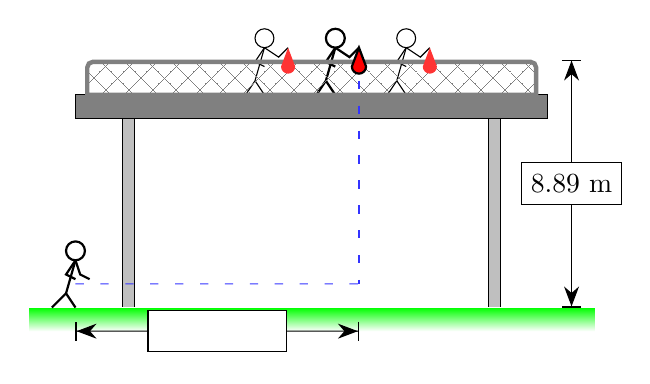
\begin{tikzpicture}[scale=0.6]
      \tikzstyle{main balloon}=[thick, fill=red]
      \tikzstyle{secondary balloon}=[draw=none, fill=red!80]
      \tikzstyle{path trace}=[
          thin,
          loosely dashed, 
          blue!80,
        ]
      \tikzstyle{ground}=[
          top color=green,
          bottom color = white,
          middle color=white,
          draw=white,
        ]
      \tikzstyle{post}=[
          fill=gray!50
        ]
      \tikzstyle{bleacher}=[
          fill=gray
        ]
      \tikzstyle{fence}=[
          draw=gray,
          ultra thick,
          pattern={Hatch[
            angle=45,
            distance={6pt},
            line width=0pt,
          ]},
          pattern color=gray,
        ]
      \tikzstyle{dist label}=[
          midway,
          fill=white,
          minimum height=1.5em,
          draw=black,
        ]
      \tikzstyle{dist arrow}=[
        {|[scale=1.5]Stealth[scale=1.5]}-{Stealth[scale=1.5]|[scale=1.5]}
        ]
      \tikzstyle{person}=[
          thick
        ]
  
      \draw (0,4) coordinate (bleacher base)
        ++ (0.25,0.5) coordinate (fence base);
      \draw[bleacher] 
        (bleacher base) rectangle ++(10,0.5);
      \draw[post] (1,0) -- 
            ++(0,4) -- 
            ++(0.25, 0) -- 
            ++ (0,-4) 
            -- cycle;
      \draw[post] (9,0) -- 
            ++(0,4) -- 
            ++(-0.25, 0) -- 
            ++ (0,-4) 
            -- cycle;
      \fill[ground] (-1,0) rectangle (11,-1);
      \draw[dist arrow] (10.5,0) -- ++ (0,5.25) node[dist label] {8.89 m}; 
  
      \begin{scope}[person]
        \draw (0,1.2) circle (0.2);
        \coordinate (waste) at (-.2,.3);
        \coordinate (neck) at (0,1);
        \draw (waste) -- (neck);
        \draw (-.5,0) -- (waste);
        \draw (0,0) -- (waste);
        \draw (neck) -- ++(.1,-.3) -- ++(.2,-.1);
        \draw (neck) -- ++(-.2,-.3) -- ++(.2,-.1);
      \end{scope}
  
      % usage: \drawdropper{x-coord}{style}{counter}
      \newcommand{\drawdropper}[3]{
        \begin{scope}[#2]
          \draw (bleacher base) ++(#1,1.5) coordinate (neck);
          \draw (neck) ++ (0,0.2) circle (0.2);
          \draw (neck) ++ (-.2,-.7) coordinate (waste);
          \draw (waste) -- (neck);
          \draw (neck) -- ++(.3,-.2) -- ++(.2,.2) coordinate(balloon #3);
          \draw (neck) -- ++(-.2,-.3) -- ++(.2,-.1); 
          \draw (waste) -- ++(0.2,-0.3);
          \draw (waste) -- ++(-0.2,-0.3);
        \end{scope}
      }
      % usage: \drawballoon{style}{counter}
      \newcommand{\drawballoon}[2]{
        \draw[#1] (balloon #2) 
          -- ++(-0.15,-0.4)
          arc[
            start angle = 180,
            end angle   = 360,
            radius      = 0.15
          ]
          -- cycle;
      }
  
      \drawdropper{5.5}{person}{1}
      \drawdropper{4.0}{person,thin}{2}
      \drawdropper{7.0}{person,thin}{3}
  
  
      \draw[fence] (fence base) 
        to[rounded corners=2pt] ++(0,.7)
        to[rounded corners=2pt  ] ++(9.5,0)
        -- ++(0,-.7)
        -- cycle;
  
      \drawballoon{main balloon}{1}
      \drawballoon{secondary balloon}{2}
      \drawballoon{secondary balloon}{3}
  
  
      \draw[path trace] (0,0.5) coordinate (start) 
        -- (balloon 1 |- start);
      \draw[path trace] (balloon 1) ++ (0,-0.7) 
        -- (balloon 1 |- start);
  
      \draw[dist arrow] (start) 
        ++ (0,-1) coordinate (below start) 
        -- (balloon 1 |- below start) 
        node[dist label, minimum width=5em] {};
  
  
    \end{tikzpicture}
  \end{center}

\paragraph{Calculation:}
  Show all your calculations below. Make sure to label each calculation with what it is that you are looking for.  Include knowns and unknowns and show all work.

  % \vspace{2em}
  % \noindent
  % \begin{tikzpicture}
  %   \begin{scope}[gray, loosely dotted, thick]
  %     \draw (3.25in,-.25in) -- (3.245in,-4.75in);
  %     \draw (0in,-3.25in) -- (6.49in,-3.25in);
  %   \end{scope}
  % \end{tikzpicture}

\pagebreak

\paragraph{Explanation:}
  In paragraph form, explain the steps you took to complete the calculation.  Be complete and detailed.
  \vspace{30em}

\paragraph{Results:}
  In paragraph form, comment on how successful you were.  Discuss any errors that came up in the lab and what you could do in the future to correct them.
  \vs


\paragraph{Grading Rubric:} \hfill
\vspace{1em}

\noindent
\begin{tabular}{
  p{.95cm}p{4.15cm}
  p{.8cm}p{3.7cm}
  p{.8cm}p{3.58cm}
}
  \hline
  $\bigcirc$ {\bf 10:} &
  Calculations are complete, correct, \& easy to follow. &
  $\bigcirc$ {\bf 7:}  &
  Calculations are difficult to follow or have errors. &
  $\bigcirc$ {\bf 5:}  &
  Calculations are incomplete or incorrect. \\\hline

  $\bigcirc$ {\bf 5:} &
  Explanations \& Results are thorough \& complete. &
  $\bigcirc$ {\bf 3:}  &
  Explanations \& Results are not detailed enough. &
  $\bigcirc$ {\bf 1:}  &
  Explanations \& Results are incomplete. \\\hline
  \multicolumn{6}{r}{}\\
  \multicolumn{6}{r}{Total Score:   \fillin[][5em]/15}

\end{tabular}

\end{document}